\documentclass{article}
\usepackage[utf8x]{inputenc}
\usepackage{amsmath}
\usepackage{anysize}
\marginsize{2cm}{1cm}{0.5cm}{1cm}
\usepackage{amsthm}
\usepackage{listings}
\usepackage{graphicx}
\usepackage{multicol}
\usepackage[spanish]{babel}
\usepackage{layout}
\usepackage{amssymb,latexsym}
\providecommand{\abs}[1]{\lvert#1\rvert}
\usepackage{color}
\usepackage[dvipsnames]{xcolor}
\usepackage{float}
\usepackage{lipsum}
\usepackage[small,labelfont=bf, margin=10pt]{caption}
\selectlanguage{spanish}
\usepackage{enumerate}
\usepackage{hyperref}
\usepackage{verbatim}
\usepackage{capt-of}
\usepackage{multirow}
\usepackage{url}
\usepackage{mathrsfs}

\title{Proyecto Final Relatividad General}
\author{David Leonardo Bernal Fino, Johan Mendez, Steven Prieto}
\date{Noviembre de 2017}

\begin{document}

\maketitle

\section{Objetivo}

El objetivo del presente trabajo consiste en encontrar el potencial efectivo para la métrica de Kerr, para órbitas ecuatoriales, y variar los parámetros de Spin, momento angular, masa, radio de Schwarzschild y momento angular para evidenciar cómo cambian las órbitas en función de éstos. 

\section{Métrica de Kerr}

Esta métrica se presenta posterior a la metrica de Schwarzschild, que es una solución estática a las ecuaciones de campo de Einstein, mientras que la métrica de Kerr representa un objeto rotante con Spin $a$ y momento angular $J$. Schwarzschild presenta una solución ampliamente aceptada debido a los efectos observables que presenta sin embargo, una interrogante que presento en su momento es que fue concebida para un objeto estático. Sin embargo, hasta donde se ha observado, todos los objetos del universo presentan una rotación por lo que fue una necesidad encontrar una métrica que describiera dicha rotación y sus efectos en el espacio-tiempo alrededor.

\medskip

La métrica de Kerr, vista por medio del elemento de línea, es la siguiente:

\begin{align*}
    ds^2=-\frac{(\Delta-a^2sen^2\theta)}{\Sigma}c^2dt^2-2\frac{r_sac}{\Sigma}rsin^2\theta d\phi dt +\frac{\Sigma}{\Delta}dr^2+\Sigma d\theta^2-\frac{\Sigma^2 sin^2\theta}{\Sigma}d\phi^2
\end{align*}

Donde los siguientes términos tienen las siguientes definiciones:

\begin{align*}
    &\Delta=r^2-2r_sr+a^2\\
    &\Sigma=r^2+a^2cos^2\theta\\
    &\Sigma^2=(r^2+a^2)^2-a^2\Delta sin^2\theta\\
    &a=\frac{J}{mc} \longrightarrow \ \text{Spin}\\
    &r_s=\frac{2mG}{c^2} \longrightarrow \ \text{Radio de Schwarzschild}
\end{align*}

Con $J$ el momento angular, $m$ la masa del agujero negro, $G$ la constante de gravitación universal y $c$ la velocidad de la luz. 

\medskip

Esta métrica presenta una enorme complejidad al momento de realizarle procedimiento alguno, de hecho en general no es posible hallar las geodésicas de forma simple usando relaciones de conservación. Por esto, se consideran únicamente las geodésicas contenidas en el plano ecuatorial $\theta=\pi/2$. Esto modifica la métrica de la siguiente manera:

\begin{align*}
    ds^2=-\frac{(r-2r_s)}{r}c^2dt^2-2\frac{r_sac}{r^2}r d\phi dt +\frac{r^2}{\Delta}dr^2-r^2d\phi^2
\end{align*}

El lagrangiano asociado a esta métrica puede expresarse como 
\begin{align*}
    \mathcal{L}=-\frac{(r-2r_s)}{r}c^2\dot{t}^2-2\frac{r_sac}{r^2}r \dot{\phi} \dot{t} +\frac{r^2}{\Delta}\dot{r}^2-r^2\dot{\phi}^2
\end{align*}

Podemos observar que las derivadas parciales de $\mathcal{L}$ respecto a $t$ y a $\phi$ son iguales a cero porque no depende explícitamente de estas variables, por lo tanto la energía y el momento canónicamente conjugado (angular) son cantidades conservadas.

Para partículas masivas $E$ y $L$ son, respectivamente, la energía y
el momento angular por unidad de masa, medido al infinito con respecto al agujero negro. Para partículas sin masa, $E$ y $L$ son la energía y el momento angular en el infinito.\\
Las ecuaciones para la métrica en el espacio-tiempo de Kerr son muy complicadas de resolver directamente, por lo que para simplificar el problema, se usan las cantidades conservadas, análogo al movimiento geodésico en el espacio-tiempo de Schwarzschild. Para esto, son necesarias cuatro relaciones algebraicas que implican $u^\mu$.
Además 
\begin{align}\label{20.10}
\mathcal{L}=g_{\mu\nu}u^\mu u^\nu=\delta    
\end{align}
donde
\begin{align*}
\begin{cases}
\delta=&-c^2=-1\qquad \text{para partículas con masa}\\
\delta=&-0\qquad\qquad\quad \text{para partículas con masa}
\end{cases}
\end{align*}

%En el espacio-tiempo de Schwarzschild una ecuación es proporcionada por la consideración de la órbita ecuatorial; en el espacio-tiempo de Kerr se considerará igualmente una órbita ecuatorial ($\theta=\pi/2$) ya que sólo para este ángulo, las órbitas son planas.

Derivando el lagrangiano respecto a $\dot{t}$ y a $\dot{\phi}$ tenemos
\begin{align}
    \frac{\partial\mathcal{L}}{\partial\dot{t}}&=-\frac{(r-r_s)}{r}c^2\dot{t}-\frac{r_sac}{r^2}r\dot{\phi}=E\\
    \frac{\partial\mathcal{L}}{\partial\dot{\phi}}&=-2r^2\dot\phi-\frac{r_sac}{r^2}r\dot{t}=L
\end{align}
o también
\begin{align}
    \frac{\partial\mathcal{L}}{\partial\dot{t}}&=\left(1-\frac{r_s}{r}\right)\dot{t}+\frac{r_sa}{r}\dot{\phi}=E\\
    \frac{\partial\mathcal{L}}{\partial\dot{\phi}}&=\left(r^2+a^2+\frac{r_sa^2}{r}\right)\dot\phi-\frac{r_sa}{r}\dot{t}=L
\end{align}
En la métrica de Schwarzschild basta con reemplazar los valores de la energía y el momento en el Lagrangiano directamente, en este caso es fácil comprobar que de hacer lo mismo, se llegará a una expresión bastante compleja de donde no se podrá despejar el término de la energía. Por lo tanto, para solucionear estas ecuaciones, usemos algunos cambios de variable
$$A=1-\frac{r_s}{r}$$
$$B=\frac{r_sa}{r}$$
\begin{align}\label{20.20}
C=r^2+a^2+\frac{r_sa^2}{r}    
\end{align}

Por lo tanto las expresiones para la energía y el momento angular se convierten en
\begin{align}\label{20.21}
    E= A\dot{t}+B\dot{\phi}
\end{align}
\begin{align}\label{20.22}
    L= C\dot\phi-B{r}\dot{t}
\end{align}

Además, se puede usar la siguiente relación
$$AC+B^2=\left(1-\frac{2r_s}{r}\right)\left(r^2+a^2+\frac{2r_sa^2}{r}\right)+\frac{4r_s^2a^2}{r^2}=r^2-2r_sr+a^2=\Delta$$
Por lo tanto

\begin{align}
    CE -BL &= [AC+B^2]\dot{t} = \Delta\dot{t}\\
    AL + BE &= [AC+B^2]\dot{\phi} = \Delta \dot{\phi}
\end{align}

Por lo tanto se puede obtener

\begin{align}
    \dot{t} &= \frac{1}{\Delta}  \left[\left(r^2+a^2+\frac{r_{s}a^2}{r}\right)E + \frac{r_{s}a}{r}L\right] \\
    \dot{\phi} &= \frac{1}{\Delta}  \left[\left(1-\frac{r_{s}}{r}\right)L + \frac{r_{s}a}{r}E\right]
\end{align}






Notemos que la cantidad C puede escribirse de diferente forma, asi

\begin{align}
    \frac{(r^2+a^2)^2-a^2\Delta}{r^2} &= \frac{1}{r^2}[(r^2+a^2)(r^2+a^2)-a^2(r^2+a^2-r_{s}r)]\\
    &= \frac{1}{r^2}[(r^2+a^2)r^2-r_{s}ra^2)] = r^2+a^2 +\frac{r_{s}a^2}{r}\\
    & \equiv C
    \label{C}
\end{align}

Se ve entonces que $C$ siempre va a ser postivo. Ahora se quiere encontrar la ecuación de la componente radial de la cuadrivelocidad. la ecuación(\ref{20.10}) puede ser reescrita en términos de $A$,$B$,$C$

\begin{align}
    g_{\mu\nu} &= \delta \\
    &= -A\dot{t}^2-2B\dot{t}\dot{\phi} +C\dot{\phi}^2 + \frac{r^2}{\Delta}\dot{r}^2\\
    &  = -(a\dot{t}+B\dot{\phi})\dot{t} + (-B\dot{t}+C\dot{\phi})\dot{\phi}+ \frac{r^2}{\Delta}\dot{r}^2\\
    & = -E\dot{t} + L\dot{\phi}+\frac{r^2}{\Delta}\dot{r}^2
\end{align}


En donde se utilizó la ecuación \ref{C}






\begin{align}
    \dot{r}^2 = \frac{\Delta}{r^2}(E\dot{t}-L\dot{\phi+\delta}) = \frac{1}{r^2}(CE^2 -2BLE -AL^2) +\frac{\delta \Delta}{r^2}
\end{align}



EL polinomio $CE^2 -2BLE -AL^2$ tiene ceros, y son los siguientes

\begin{align}
V_{+-} = \frac{BL \pm \sqrt{B^2L^2 +ACL^2}}{C} = \frac{L}{C}(B\pm \sqrt{\Delta})
\end{align}




\begin{align}
    \dot{r}^2 = \frac{C}{r^2}(E-V_{+})(E-V_{-})+ \frac{\delta \Delta}{r^2}
\end{align}



\begin{align}
    \dot{r}^2 = \frac{C}{r^2}(E-V_{+})(E-V_{-})+ \frac{\delta \Delta}{r^2}
\end{align}




\begin{align}
    \dot{r}^2= \frac{(r^2+a^2)^2-a^2\Delta}{r^4}(E-V_{+})(E-V_{-})
\end{align}



\begin{align}
    V_{\pm} = \frac{r_{s}ar\pm r^2 \sqrt{\Delta}}{(r^2+a^2)^2 -a^2\Delta}L
\end{align}

Finalmente se tiene el potencial que se va a graficar, y el cual se varían los parámentros

\begin{align}
    V_{\pm} =\frac{2Lr \pm r^2\sqrt{r^2-2r_{s}r+4L^2/r_{s}^2}}{r^4+4(r/r_{s})^2L^2+8(r/r_{s})L^2}L
\end{align}

Se realizaron graficas del potencial usando solo la raiz positiva ($v_+$), bajo los siguientes parámetros:

\begin{figure}[H]
\centering
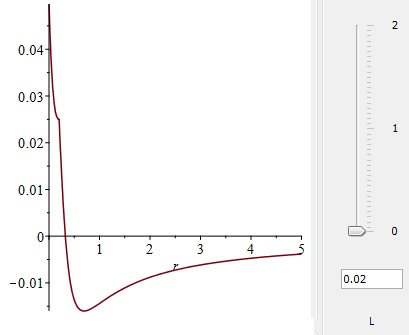
\includegraphics[scale=0.7]{rs=02,L=002.jpg}  \caption{Gráfica del potencial para un radio de Schwarzschild igual a $0.2$ y un momento angular de$0.002$}\label{002}
\end{figure}

\begin{figure}[H]
\centering
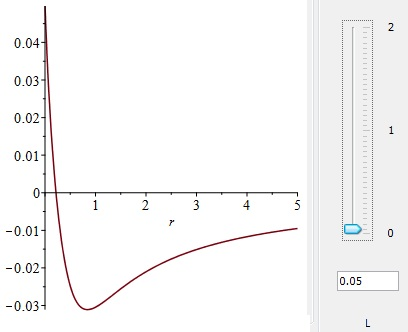
\includegraphics[scale=0.7]{rs=02,L=005.jpg}  \caption{Gráfica del potencial para un radio de Schwarzschild igual a $0.2$ y un momento angular de$0.005$}\label{005}
\end{figure}

\begin{figure}[H]
\centering
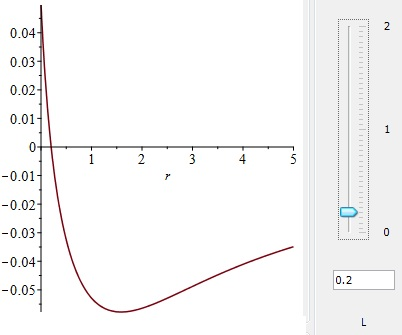
\includegraphics[scale=0.7]{rs=02,L=02.jpg}  \caption{Gráfica del potencial para un radio de Schwarzschild igual a $0.2$ y un momento angular de$0.02$}\label{02}
\end{figure}

\begin{figure}[H]
\centering
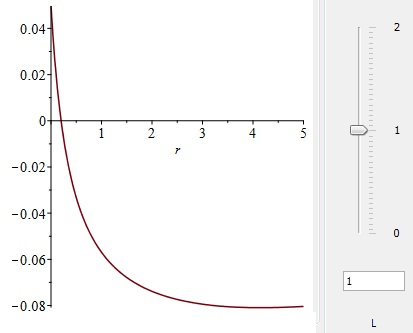
\includegraphics[scale=0.7]{rs=02,L=1.jpg}  \caption{Gráfica del potencial para un radio de Schwarzschild igual a $0.2$ y un momento angular de$0.1$}\label{1}
\end{figure}

Vemos que para momento angular (pequeño) la gráfica tiende a ser tipo Newton la cual cae en el origen. Sin embargo, mientras crece, el mínimo desaparece hasta tomar una forma tal que toda partícula sin importar con la energía que venga, golpea con el potencial y se devuelve o llega hasta $r=0$.

Por último, se encontro la siguíente particularidad para cuando el término $-2r r_s$ supera el término $r^4$ dentro de la raiz en el potencial, la gráfica parece ''romperse":

\begin{figure}[H]
\centering
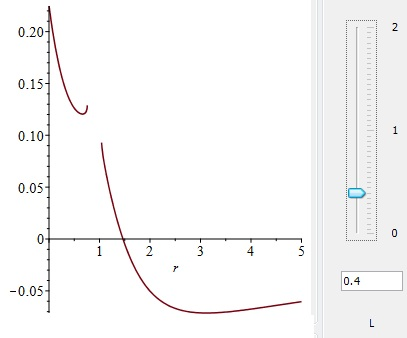
\includegraphics[scale=0.7]{mistake.jpg}  \caption{Gráfica del potencial ''roto"}\label{m}
\end{figure}

\begin{equation}
    2r r_s>r^4 \Rightarrow V\in \mathbb{C}
\end{equation}

\section{Referencias}

\begin{thebibliography}{99}

\bibitem{im} \textit{Geodesic motion in Kerr spacetime, Chapter 20}
\url{http://www.roma1.infn.it/teongrav/VALERIA/TEACHING/ONDE_GRAV_STELLE_BUCHINERI/AA2010_2011/LEZIONI_MIE_BH/kerrgeod.pdf}

\bibitem{im2} \textit{The Kerr solution, Chapter 19}
\url{http://www.roma1.infn.it/teongrav/VALERIA/TEACHING/ONDE_GRAV_STELLE_BUCHINERI/AA2010_2011/LEZIONI_MIE_BH/kerr.pdf}

\bibitem{dos} \textit{Equatorial circular motion in Kerr spacetime} \url{https://arxiv.org/pdf/1105.2959.pdf}

\end{thebibliography}

\end{document}
